% Journal-neutral source. Edit this file directly.
\documentclass[11pt,a4paper]{article}
\usepackage[T1]{fontenc}
\usepackage[utf8]{inputenc}
\usepackage[english]{babel}
\usepackage[margin=25mm]{geometry}
\usepackage{amsmath,amssymb,graphicx}
\usepackage{placeins}
\usepackage[numbers,sort&compress]{natbib}
\usepackage[hyphens]{url}
\usepackage[hidelinks]{hyperref}
\ifx\pdfmapfile\undefined\else
\pdfmapfile{+cm-super-t1.map}\pdfmapfile{+cm-super-ts1.map}\fi
\setlength{\emergencystretch}{2em}
\renewcommand{\topfraction}{0.85}
\renewcommand{\textfraction}{0.10}
\renewcommand{\floatpagefraction}{0.75}

\title{Stress transfer and dislocation response near a constrained
Al$_{13}$Fe$_4$ inclusion in aluminium}
\author{I.~Mikhailovskiy\thanks{Corresponding author.
\texttt{ilyamihailovsy@gmail.com}} \and D.~Pshonkin}
\date{Moscow Polytechnic University, Moscow, Russia}

\begin{document}
\maketitle

\begin{abstract}
The mechanical response to a prescribed deformation of an Al$_{13}$Fe$_4$
inclusion in aluminium was examined using atomistic calculations. A ridge
in a 91\,428-atom interface cell was elongated by 0.194\% and restrained
while the matrix relaxed. The additional shear stress reached a magnitude of
15.45~MPa above the ridge axis, with substantial cancellation upon
averaging across the cell. In matched loading runs, the upper-dislocation
departure criterion is met one saved frame apart. A single pair of
trajectories is insufficient to establish a systematic effect of inclusion
deformation on dislocation motion. A separate activated-glide model
quantifies the sensitivity of creep to the assumed stress amplitude and
activation volume. The calculations establish a conditional mechanical
response; magnetic deformation of the inclusions and persistence after
field removal remain untested.
\end{abstract}

\noindent\textbf{Keywords}\quad molecular dynamics; interfacial stress;
dislocations; aluminium alloys; constrained deformation

\section{Introduction}

Changes in the plastic response of aluminium alloys after magnetic exposure
motivate the examination of mechanical interactions between inclusions and
dislocations. Experiments on heterogeneous Al--Mg--Si alloys containing
iron-bearing inclusions reported changes in creep after exposure to a
static field \cite{Skvortsov2019JAP,Skvortsov2019PSS,Friha2024JMMM}.
In these experiments the treatment and mechanical loading were separated
in time. Subsequent work also reported changes in transient creep and
stress relaxation \cite{Nikolaev2025SciRep}. Any explanation of the retained
response therefore requires a material state that persists after the
treatment has ended.

A possible contribution is the stress generated when an inclusion changes
shape within the surrounding matrix. Magnetostriction could provide the
deformation if the inclusion contains an appropriate magnetic constituent.
Its mechanical consequences depend on particle shape, elastic
accommodation and crystallographic orientation. A scalar estimate of
interfacial stress does not determine the shear acting on a particular
dislocation. The pre-existing interface field and the distribution of
obstacles also affect the response of a line placed near the inclusion.

The present calculations address the mechanical part of this problem using
an aluminium matrix and an Al$_{13}$Fe$_4$ inclusion. We prescribe
an inclusion elongation of 0.194\% and calculate the matrix response.
This value follows the modelling estimate associated with the earlier
147~MPa stress scale \cite{Friha2024JMMM}; it has not been measured for the
inclusions under magnetic exposure. The applied constraint fixes reference
coordinates for the inclusion atoms. Consequently, the resulting field is
the response to a specified mechanical boundary condition. Whether the
imposed deformation represents magnetostriction of real inclusions requires
separate verification.

The study combines a paired static stress calculation with trajectories of
existing dislocations in the same interface geometry. Attention is given
to the distinction between signed shear near the inclusion axis and
averages across the simulation cell. The trajectories are examined through
their initial relaxation, subsequent motion and interaction with the
periodic seam. A separate activated-glide estimate then relates assumed
stress amplitudes to a conditional change in creep rate.

\section{Methods}

\subsection{Geometry and imposed deformation}

Calculations used LAMMPS, release 22 July 2025, with KOKKOS/CUDA acceleration
\cite{Thompson2022LAMMPS} and the Al--Si--Mg--Cu--Fe second-neighbour
modified embedded-atom potential of Jelinek et al.\ \cite{Jelinek2012}.
The face-centred cubic aluminium matrix has lattice parameter
$a_0=4.05$~\AA{} and axes
$x\parallel[1\bar{1}0]$, $y\parallel[11\bar{2}]$ and
$z\parallel[111]$. This orientation places a (111) glide plane parallel
to the nominal interface and its $[1\bar{1}0]$ glide direction along $x$.
An edge line parallel to $y$ then carries Burgers vector
$\mathbf b=(a_0/2)[1\bar{1}0]$, with magnitude $b=2.864$~\AA{}.

The monoclinic Al$_{13}$Fe$_4$ structure \cite{Liu2024CIF} forms a
20~\AA{} support layer topped by a half-elliptical ridge with semi-axes
35~\AA{} along $x$ and 20~\AA{} along $z$. The ridge spans the periodic
$y$ direction. The interface cells contain 91\,428 atoms, comprising
72\,532 matrix atoms and 18\,896 inclusion atoms. Their in-plane dimensions
are $154.64\times64.48$~\AA$^2$. Periodic boundaries apply along $x$
and $y$; the upper aluminium surface faces vacuum and the bottom
6~\AA{} is fixed. Figure~\ref{fig:model} shows the geometry. Interfacial
bonding and any atomic rearrangement across the interface are governed by
the interatomic potential.

\FloatBarrier
\begin{figure}[!htbp]
\centering
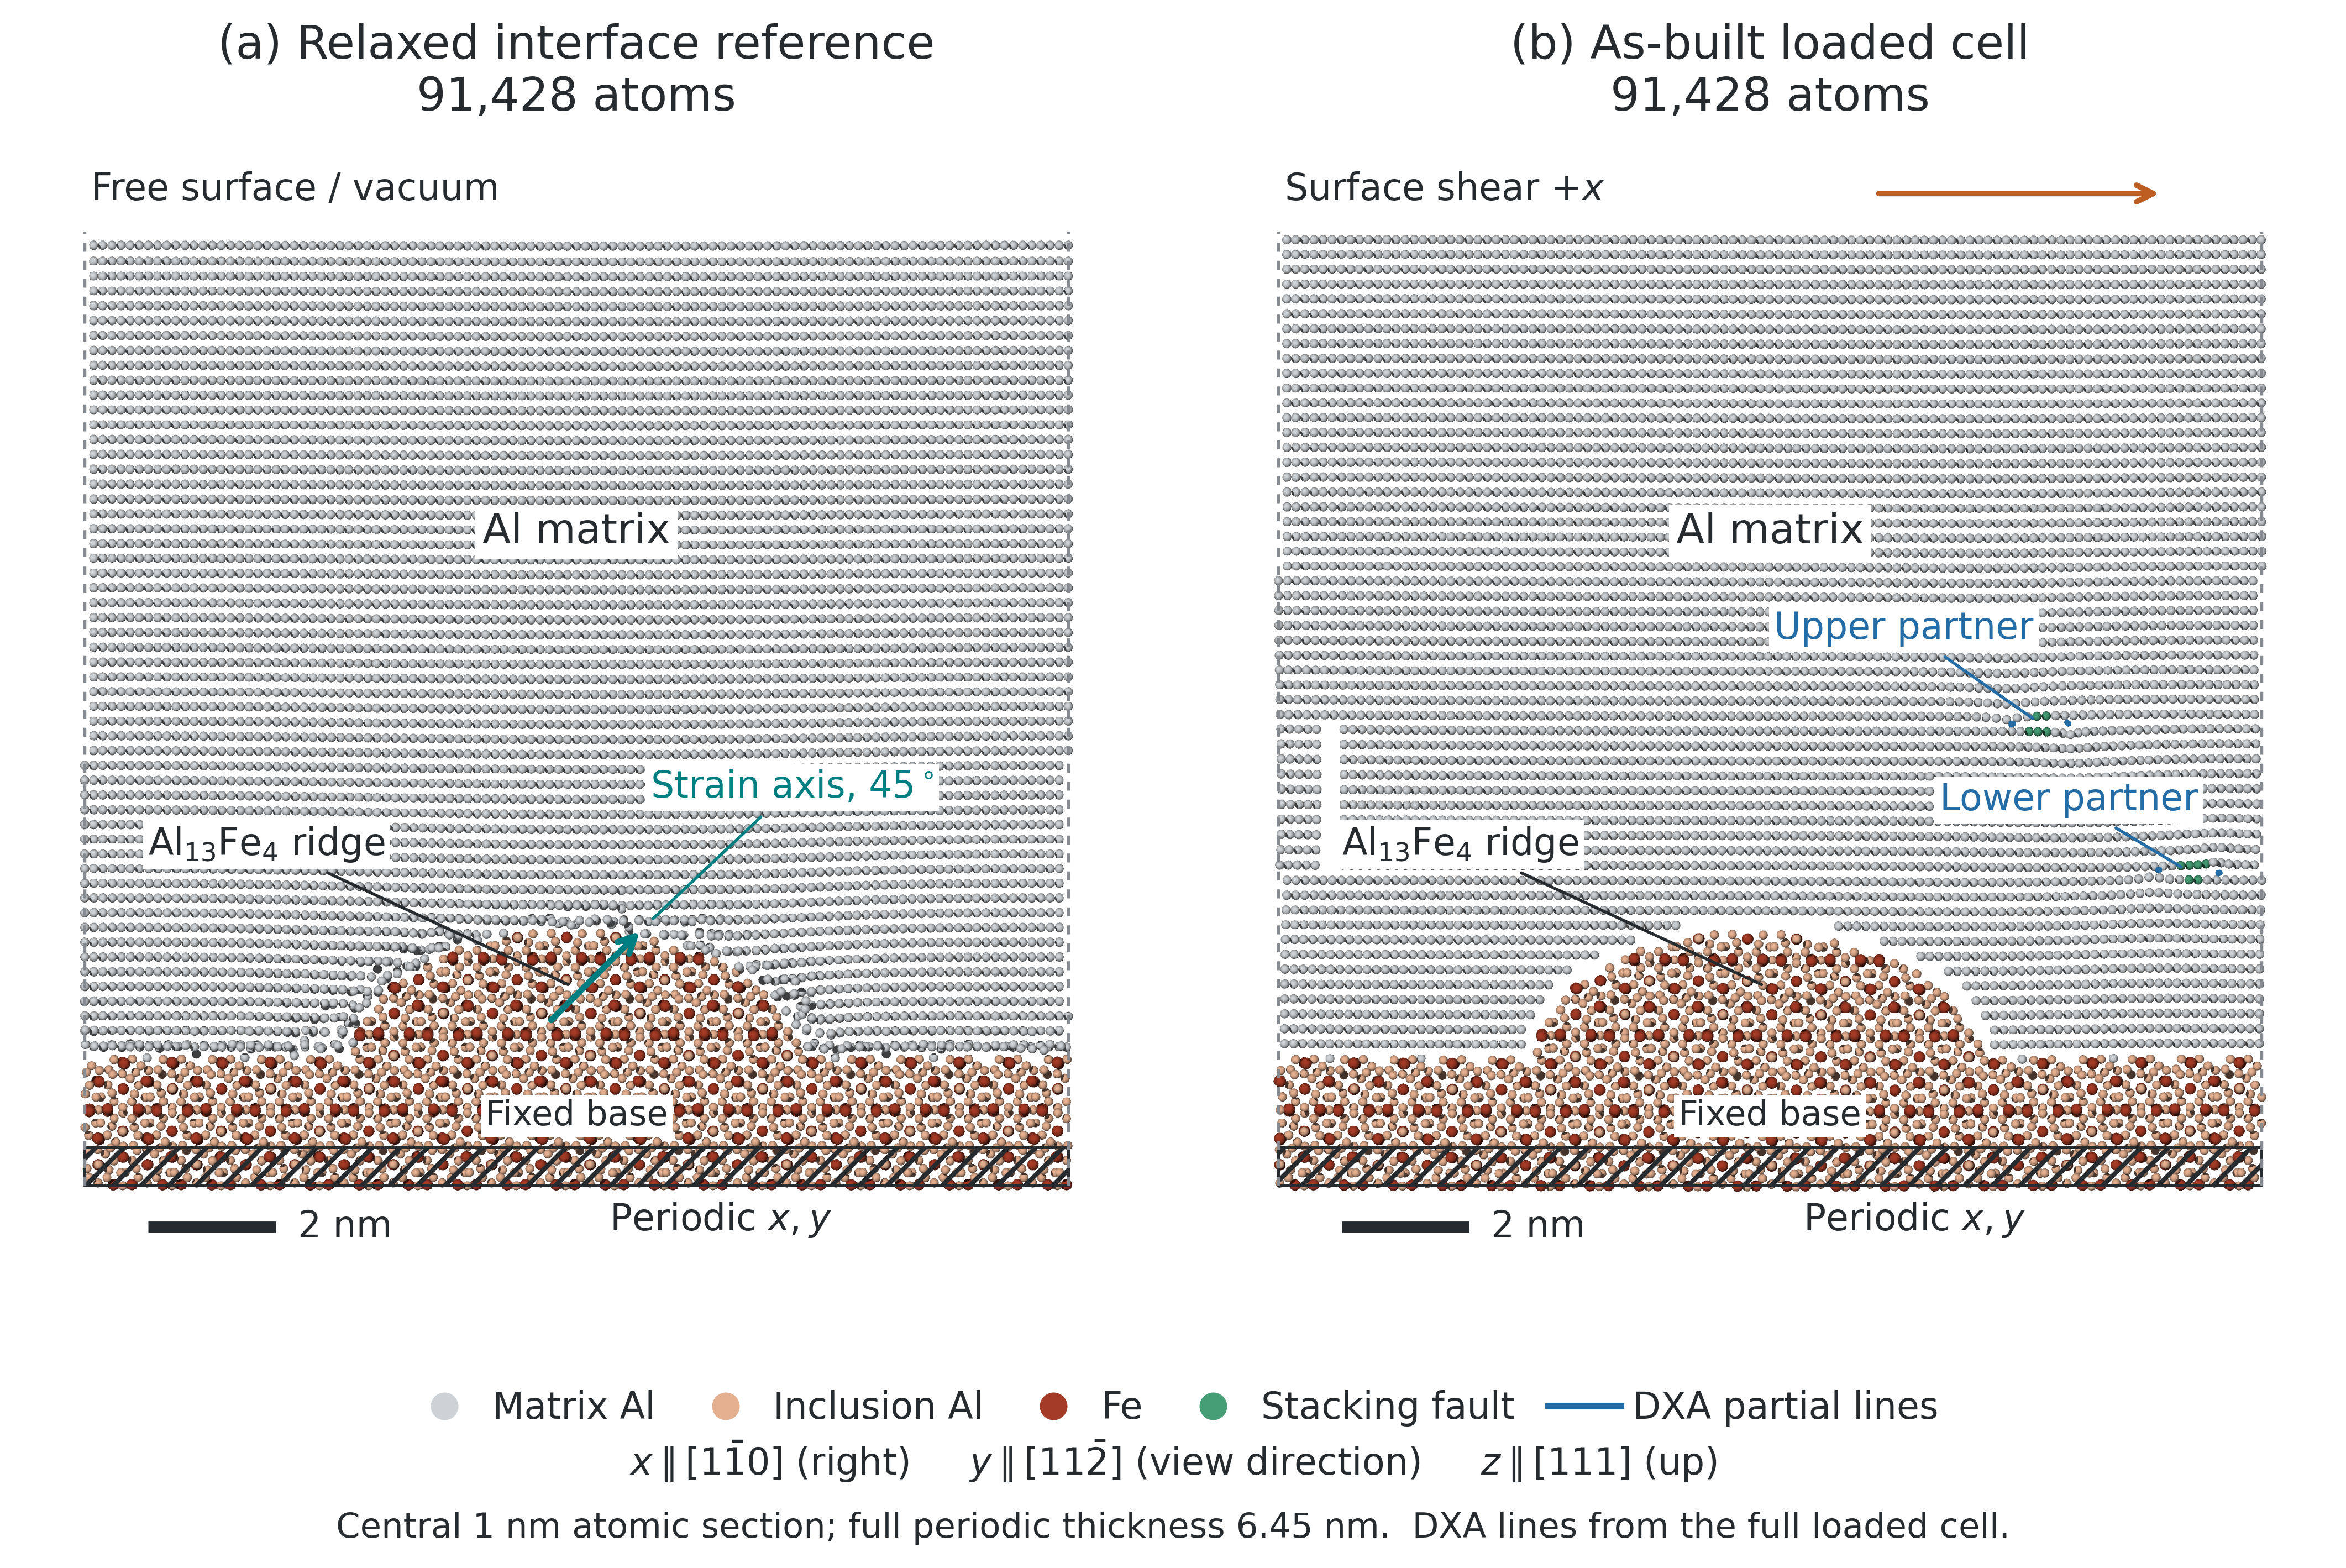
\includegraphics[width=0.92\linewidth]{fig_model.png}
\caption{Atomistic interface geometry rendered from LAMMPS configurations
with OVITO. The Al$_{13}$Fe$_4$ ridge extends along $y$ above a flat
support layer. The coordinate axes identify the glide direction, line
direction and interface normal. The loaded configuration includes an
oppositely signed edge-dislocation pair. The upper layers transmit the
applied shear and the bottom layer is fixed.}
\label{fig:model}
\end{figure}
\FloatBarrier

The ridge atoms are displaced about their centroid using the small-strain
tensor
\begin{equation}
\mathbf E_0=\frac{3\varepsilon_0}{2}
 \left(\mathbf u\otimes\mathbf u-\frac{\mathbf I}{3}\right),
\qquad
\varepsilon_0=0.00194,\qquad
\mathbf u=\frac{(1,0,1)}{\sqrt{2}} .
\label{eq:strain}
\end{equation}
Its zero trace conserves volume to first order. The chosen direction
maximises the imposed $xz$ shear component, $E_{0,xz}=0.001455$, within
this family of deformations. It defines one favourable orientation.
The support layer receives no imposed displacement.

Preparation includes conjugate-gradient minimisation, 6~ps at 300~K,
12~ps of cooling to 0.5~K and a final minimisation. Both static configurations
are constructed from one relaxed control structure, preserving atom
identities. Inclusion atoms are attached to their respective reference
coordinates by harmonic springs of stiffness $20$~eV/\AA$^2$, while the
matrix remains free to relax. The two copies are minimised with identical
settings and both reach the requested force two-norm of 0.02~eV/\AA{}.
This comparison uses one prepared state; sensitivity to initial structure
and minimisation tolerance has not been established.

The potential is unchanged, so the springs supply the forces that maintain
the deformation. A material eigenstrain would alter the stress-free state
of the inclusion. Spring reactions remain part of the paired response.
Full preparation and convergence information is given in the
Supplementary Information.

\subsection{Stress and dislocation measurements}

The six components of the configurational atomic virial are averaged
before forming stress invariants. The conversion uses the aluminium atomic
volume $16.61$~\AA$^3$. Profiles compare the perturbed and control tensors,
$\Delta\boldsymbol\sigma=\boldsymbol\sigma_\varepsilon-
\boldsymbol\sigma_0$, in layers 4~\AA{} thick. The stored tensor uses
positive normal stress in compression. The tensor has the opposite sign to
the tensile-positive Cauchy convention. Reversing its sign leaves absolute
resolved shear stresses and the von Mises stress unchanged.
The coordinate $r=z-20$~\AA{}
measures height above the nominal interface plane; $d=r-20$~\AA{} is
height above the nominal ridge crest. For a layer spanning the cell,
$d$ is not a nearest-surface distance.

Two spatial averages are retained, across the full cell width and within
$|x-x_c|<10$~\AA{} of the ridge axis. Layers intersecting the inclusion
are excluded from the matrix profile. The signed shear on the selected
$(111)[1\bar{1}0]$ system is $\Delta\sigma_{xz}$. The supplementary scalar
$\mathrm{RSS}_{\max}$ is the maximum of
$|\mathbf s\cdot\Delta\boldsymbol\sigma\mathbf n|$ over the twelve fcc
slip systems, with unit slip direction $\mathbf s$ and plane normal
$\mathbf n$.

Layer membership and the axial window are defined by control coordinates
and applied to the same atom identities in both snapshots. This
construction avoids changing the sampled population as atoms move across
layer boundaries. The retained layers lie entirely above every inclusion
atom in both snapshots and contain only matrix aluminium, identified by
atom ID. No thermal kinetic
term enters the minimised profiles. The von Mises stress of the
difference tensor and the difference between two von Mises stresses are
distinct quantities; only the former describes the shear invariant
of the perturbation.

The loaded interface cells also contain 91\,428 atoms. Two oppositely
signed edge lines are inserted on parallel glide planes separated by
23.4~\AA{}, with an initial horizontal offset of the same magnitude.
Their motion is followed using the dislocation extraction algorithm
(DXA) \cite{Stukowski2012DXA} in OVITO \cite{Stukowski2010OVITO}.
Dynamics uses a 1~fs step and a 300~K Nos\'e--Hoover thermostat.
After 5~ps without applied shear, forces on the upper atomic layers
increase according to a ramp whose rate is smoothly introduced over
16~ps. The matched restrained runs end at nominally 145.45~MPa.
An additional unstrained run with an unrestrained inclusion extends to
400~MPa. Analysis samples are spaced by 2~ps, corresponding to approximately
9.09~MPa in the linear part of the ramp.

Line positions are unwrapped along the periodic $x$ direction and grouped
by Burgers-vector family. For an individual line, a linear baseline is
fitted to available positions from 4~ps onward while the nominal stress
is below 40~MPa. Departure requires a deviation larger than six times
the baseline residual standard deviation, with a minimum of 8~\AA{},
and persistence in the next two available sampling positions. The stored
detector also accepts a missing line at a following frame. Accordingly,
line continuity is examined alongside this numerical criterion, especially
when a segment reaches the periodic seam. Quoted intervals represent
sampling brackets rather than confidence intervals.

A separate 92\,800-atom alloy cell provides a contextual mobility
comparison. It contains 1.0~at.\% Mg and 0.6~at.\% Si and no inclusion.
Its distinct geometry and stepwise loading are documented in the
Supplementary Information. This comparator is not included in the
matched interface calculation.

\section{Results}

\subsection{Stress transferred to the matrix}

The unstrained interface already supports a substantial residual stress.
In the nearest retained layer, at $d=2$~\AA{}, the control von Mises
stress is approximately 850~MPa. The next three layers give 106, 185 and
157~MPa. Such spatially averaged atomic stresses reflect the assembled
interface and its relaxed atomic structure. Their magnitudes cannot be
equated directly with a macroscopic uniaxial yield stress. The non-monotonic
near-interface profile also prevents extraction of a unique decay length
from the absolute stress alone.

The imposed perturbation produces a smaller change superposed on that
background (Fig.~\ref{fig:field}). The signed axial-window shear is negative throughout the
retained profile, reaching $-15.451$~MPa at $d=22$~\AA{}. Its magnitude
is about 11--15~MPa over the sampled interval $d=2$--30~\AA{}, then falls
to 10.258~MPa at 46~\AA{}, 5.139~MPa at 66~\AA{} and 1.905~MPa at
86~\AA{}. These values describe spatial attenuation in a minimised
configuration. They contain no measurement of a relaxation time.

Across the full width, the signed shear is mostly positive and reaches
5.042~MPa at $r=50$~\AA{}. Its different sign and smaller magnitude show
that the averaging region changes the mechanical quantity being
reported. At $r=46$~\AA{}, the width-averaged $xz$ component nearly
cancels, while $\mathrm{RSS}_{\max}=0.558$~MPa occurs on
$(111)[01\bar{1}]$. The nearest layer, at $r=22$~\AA{}, instead selects
$(1\bar{1}\bar{1})[101]$ and gives the largest width-averaged
$\mathrm{RSS}_{\max}$, 5.651~MPa. The remaining layers select
$(111)[1\bar{1}0]$. The local minimum is therefore partly a consequence
of tensor projection and spatial averaging.

\FloatBarrier
\begin{figure}[!htbp]
\centering
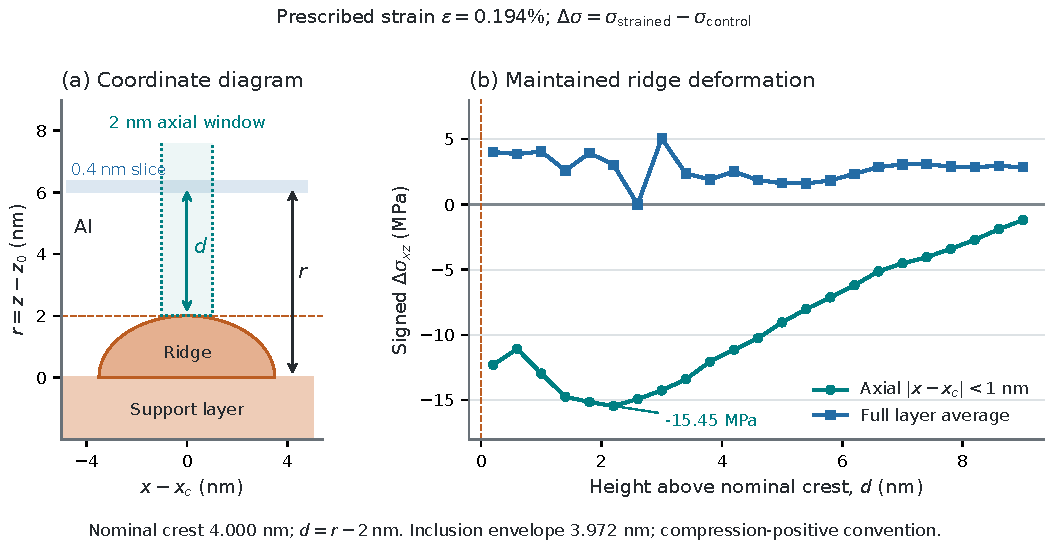
\includegraphics[width=0.96\linewidth]{fig_field.pdf}
\caption{Distance convention and signed shear in the paired minimised
configurations. The coordinate diagram defines $r$ from the flat
interface and $d$ from the nominal ridge crest at $z=40$~\AA{}.
The stress panel compares $\Delta\sigma_{xz}$ in the 20~\AA{}
axial window with its average across the cell width. Only layers
whose lower edge lies above all inclusion atoms in both snapshots
($z_{\max}=39.719$~\AA{}) are retained. The compression-positive
convention is used. The opposite signs show the
sensitivity of the reported stress to the averaging region.}
\label{fig:field}
\end{figure}
\FloatBarrier

In the thirteen layers at $r>60$~\AA{}, the width-averaged
$\mathrm{RSS}_{\max}$ has mean 2.477~MPa and standard deviation
0.543~MPa. These are spatial statistics of this configuration. They
provide no independent estimate of numerical noise or a detection limit.
The small rise in the width average at larger distances accompanies a
continued decrease of the axial-window magnitude. A finite slab and its
free surface can influence this profile, and the available calculation
does not separate their contributions. No vanishing-field distance is
assigned.

An affine fit to the iron sublattice above the support gives a projection
of 0.9728 onto the imposed ridge deformation, with formal fit standard
error 0.0038. The springs thus maintain most of the selected deformation
through matrix relaxation. The fit error describes residuals within one
configuration and cannot represent uncertainty across independent
simulations. A continuum comparison using a spherical inclusion with the
same nominal tensor and identical isotropic elastic constants inside and
outside gives an interior maximum resolved shear of 41.45~MPa
\cite{Eshelby1957}. This separate boundary-value problem provides a
reference stress scale. It supplies no upper bound for the constrained
atomistic ridge, whose support layer, free surface and spring reactions
are absent from the sphere model.

\subsection{Existing dislocations during loading}

The pre-existing lines change position during the start of all three
ramps. Figure~\ref{fig:dynamics} shows the matched restrained
upper-line histories. In the unrestrained control, the upper
line moves approximately 38~\AA{} towards the ridge axis during the first
6~ps. In the restrained control and perturbed cells, the corresponding
displacements are 31.0 and 33.2~\AA{}. The upper line then lies within
about 7--10~\AA{} of the axis. Loading starts at 5~ps, so this initial
motion occurs predominantly during preconditioning and the smooth onset
of the load.

These displacements demonstrate that the inserted pair is not stationary
in its initial environment. Residual interface stresses, interaction
between the lines, periodic images and boundary forces are all present.
Because both restrained configurations move substantially at the outset,
their later response must be interpreted relative to the relaxed line
positions. The early interval does not isolate motion caused solely by
the imposed ridge deformation.

For the upper line, departure from its low-stress trend is detected at
113.6~MPa in the restrained control and 122.7~MPa in the perturbed cell.
The preceding sampled stresses are 104.5 and 113.6~MPa, respectively.
Thus the criterion is crossed in adjacent sampling intervals. Each
configuration has only one trajectory at one loading rate. This
observation leaves the size and reproducibility of a deformation-induced
shift unresolved. A statistical null effect or a material critical stress
cannot be extracted from it.

The lower line in both restrained runs is no longer separately identified
by 10~ps. Later DXA segments appear near the periodic seam. Assigning these
segments to the original line by Burgers-vector family alone would create
a spurious late departure event. At the final analysed time of 44~ps,
about 140.9~MPa, the perturbed cell has no extracted segment. The control
retains three segments with combined length 39.3~\AA{} near
$x=7$--10~\AA{}. Their presence precludes describing both configurations
as dislocation-free. Short segments are reported as local DXA signals
without identifying a nucleation mechanism.

In the unrestrained control, the lower line crosses the motion criterion
between 95.5 and 104.5~MPa. The analysed trajectory extends to
395.45~MPa at 100~ps. No newly formed, persistent interface dislocation is
confirmed within those sampled configurations. Short signals also occur
at the periodic seam at higher loads. The nominal run endpoint is
400~MPa, beyond the last analysed regular frame. This single run gives a
restricted observation of interface activity under its own boundary
conditions; it does not measure a universal nucleation threshold.

\FloatBarrier
\begin{figure}[!htbp]
\centering
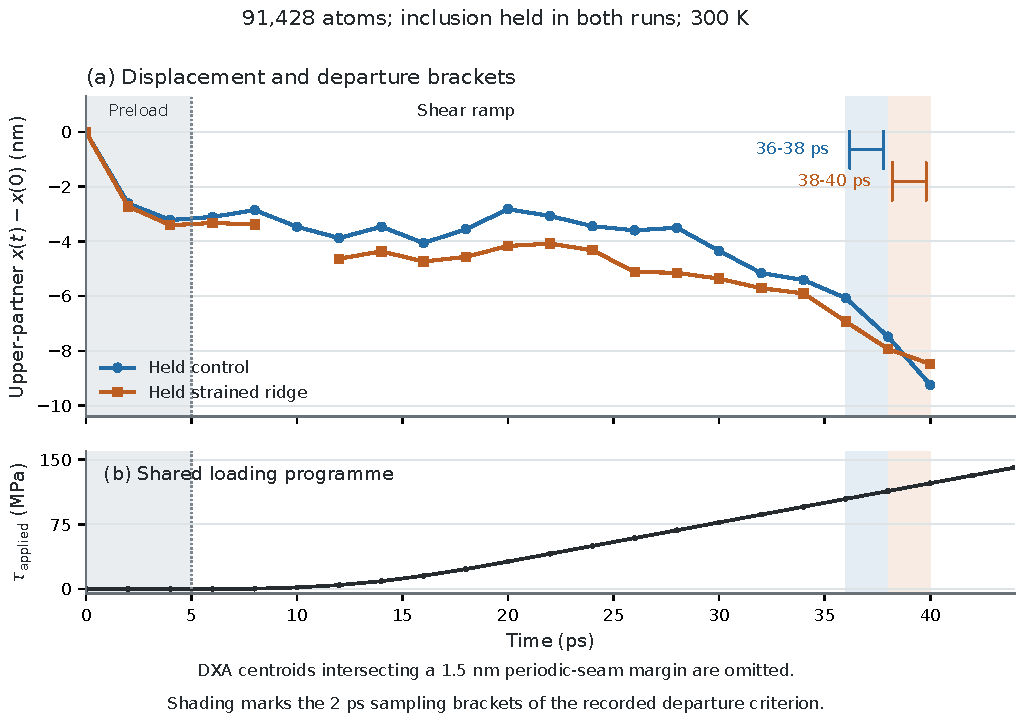
\includegraphics[width=0.96\linewidth]{fig_dynamics.pdf}
\caption{Existing-line motion in the interface cells. Upper-line positions
are followed through preconditioning and shear loading, with the applied
stress shown alongside. The restrained control and perturbed cases cross
the departure criterion one saved frame apart. The initial motion towards
the ridge and the retained DXA segments at the periodic seam constrain
interpretation of the later trajectories. Segment disappearance or
reassignment is not evidence of a new interface dislocation.}
\label{fig:dynamics}
\end{figure}
\FloatBarrier

\section{Conditional connection to creep}

A scalar activated-glide model is used to examine the consequences of the
computed stress scale. It assumes dilute compact particles with exterior
shear amplitude $\tau(R)=\tau_m(a/R)^3$, where $R$ is measured from a
particle centre. Positive and negative local stresses are assigned equal
weights, and their effect on an elementary activated rate is represented
by $\cosh(V^*\tau/k_{\mathrm B}T)$
\cite{CaillardMartin2003}. Here $V^*$ describes the stress sensitivity
of the activation barrier. These assumptions give the fractional rate
increase
\begin{equation}
H=f x\int_0^x\frac{\cosh u-1}{u^2}\,\mathrm du,
\qquad x=\frac{V^*\tau_m}{k_{\mathrm B}T},
\label{eq:bridge}
\end{equation}
to leading order in inclusion volume fraction $f$. The tensor field,
grain orientations and interactions between particles are reduced to
a single assumed amplitude.

The model evaluation uses $T=300$~K and inclusion volume fraction
$f=0.00246$. A target $H=0.25$ serves as a reference motivated by the scale
of the reported creep changes. Activation volumes from $19b^3$ to
$142b^3$ are explored as a sensitivity range. The value $70b^3$, reported
for a differently processed Al--Mg--Si alloy
\cite{Soula2022JALCOM}, provides context for that range.
No activation volume is determined by the present trajectories.

The chosen fraction corresponds approximately to a model mass fraction of
0.35\% with assumed inclusion and matrix densities of 3.85 and
2.70~g/cm$^3$, respectively. These inputs describe a representative
dispersion and carry their own compositional uncertainty. Moreover,
$H$ is a rate change in the activated model. Relating it to accumulated
experimental creep also requires a loading history over which that rate
description applies. Treating the experimental change as a fixed target
therefore introduces a second level of modelling beyond the atomistic
stress calculation.

\FloatBarrier
\begin{figure}[!htbp]
\centering
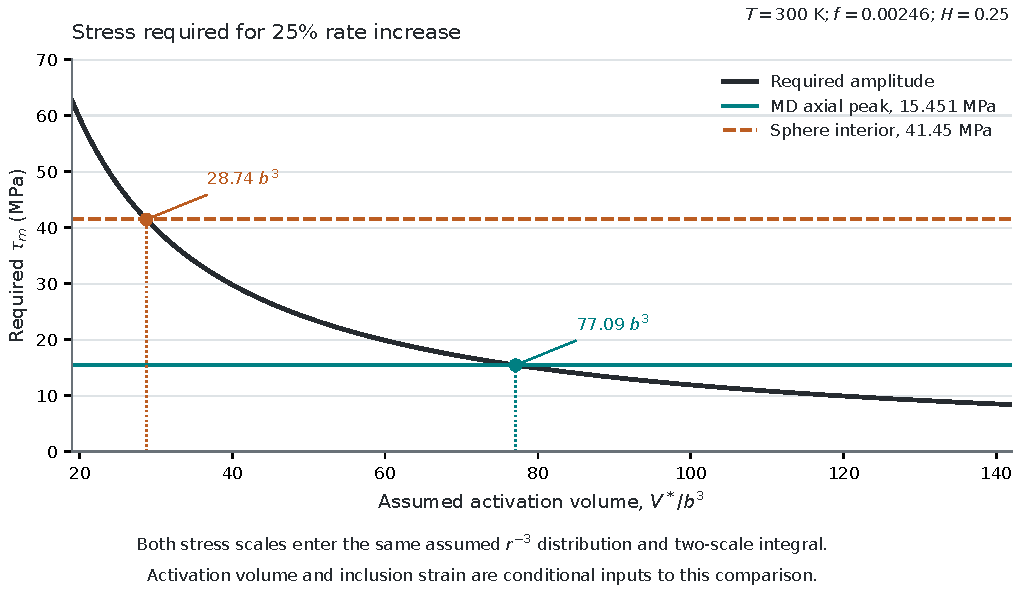
\includegraphics[width=0.92\linewidth]{fig_bridge.pdf}
\caption{Shear-stress amplitude required for a modelled 25\% creep-rate
increase as a function of activation volume at $T=300$~K and $f=0.00246$.
The curve is calculated from Eq.~\eqref{eq:bridge}. Horizontal lines mark
two illustrative amplitudes: 15.451~MPa above the ridge axis and
41.45~MPa inside the sphere. Their use in the scalar spatial model is
an additional assumption.}
\label{fig:bridge}
\end{figure}
\FloatBarrier

Solving Eq.~\eqref{eq:bridge} gives required amplitudes from 62.69 to
8.39~MPa as $V^*$ increases across the selected range
(Fig.~\ref{fig:bridge}). If 15.451~MPa is inserted as a representative
amplitude, $H=0.25$ occurs at $V^*=77.09b^3$. Using 41.45~MPa instead
gives $28.74b^3$. The conditional range for these inputs is therefore
about 29--77$\,b^3$. At $70b^3$,
the 15.451~MPa scenario gives $H=0.156$.

The axial ridge maximum and the sphere interior value belong to different
physical and spatial definitions. Substituting either into
Eq.~\eqref{eq:bridge} tests the consequences of an assumed amplitude;
it does not establish the exterior surface stress of real particles.
The exponential dependence on $V^*\tau_m$ permits the target change to be
obtained by many combinations of uncertain inputs. Agreement at a
selected activation volume therefore supplies no independent validation
of a magnetic mechanism.

\section{Discussion}

The paired static calculation quantifies how a specific constrained
deformation changes the matrix stress. Retaining its sign reveals
opposing contributions that are obscured in a full-width scalar
average. This distinction matters when assessing force on a dislocation
whose position selects only part of the field. At the height reached by
the upper line after preconditioning, the axial-window shear change
is approximately 13--14~MPa. Its scale is comparable to the separation
between sampled departure stresses. A dedicated series of trajectories
would be required to distinguish systematic changes from sensitivity
to initial state and line identification.

The current model includes several restrictions on that interpretation.
The ridge is extended periodically along the line direction and rests on
a constrained support. It does not represent an isolated particle in a
macroscopic polycrystal. The interaction potential has broad elemental
coverage, but transferability to this interface, its defect cores and
solute interactions has not been independently established here.
No cell-size study, loading-rate series or ensemble of velocity seeds
supports extrapolation of the recorded departure stresses. The thermostat
also acts during loading, so these runs do not determine adiabatic heating
or the heat-release changes measured experimentally.

The nanometre span of the present profile is tied to the imposed ridge
dimensions and to the finite simulation domain. Elastic inclusion
solutions organise distance through the ratio of separation to particle
size. A larger geometrically similar particle can therefore act over a
larger absolute distance at the same dimensionless strain. Applying that
scaling to this particular constrained ridge requires further checks of
geometry and boundary effects. The calculated profile alone cannot
establish stress overlap between inclusions several micrometres apart.

The alloy comparator adds evidence of limited line mobility in one
random solute configuration. The tracked line accumulates 1.98~\AA{}
net displacement during the completed loading history through 75~MPa,
below one Burgers-vector magnitude. The preparation minimisation did not
reach the requested force tolerance. This trajectory is therefore used
only as a supplementary observation, not as a quantitative measure of
pinning. Its configuration, time window and
internal stresses differ from those of the interface runs. It therefore
provides no transferable pinning constant or calibration of $V^*$.
The trajectory, analysis procedure and limitations of the comparator
are described in the Supplementary Information.

Connecting the imposed deformation to magnetism remains a separate
question. Studies of Al$_{13}$Fe$_4$ report weak or unusual paramagnetic
behaviour rather than establishing the strongly ferromagnetic response
assumed for some iron-bearing inclusions
\cite{Albedah2015Mossbauer,Avers2025Crystals}. The phase composition,
magnetic response and field-induced shape change of the actual inclusions
need to be established together. The chosen interatomic potential and
coordinate restraints supply no magnetic constitutive relation.
Consequently, neither the prescribed strain nor the calculated stress is
a measurement of magnetostriction.

The experimental sequence also places a temporal condition on any
mechanism. Creep is measured after magnetic exposure, whereas the static
calculation maintains the mechanical constraint and the dynamic runs
do not reproduce its removal followed by delayed loading.
Irreversible defect rearrangement, retained deformation and changes
in obstacle populations could each alter the subsequent response,
but the calculations do not establish which process accounts for the
memory. The results identify
mechanical quantities that such an explanation would need to reproduce.
They leave the origin and lifetime of the experimental memory open.

\section{Conclusions}

A constrained 0.194\% deformation of an Al$_{13}$Fe$_4$ ridge produces
a signed axial shear change with peak magnitude 15.45~MPa in the
91\,428-atom interface cell. Spatial cancellation lowers the
full-width response and changes its sign. The sampled axial magnitude
decreases to about 2~MPa at a height of 8.6~nm above the crest.

The matched loading trajectories show substantial initial motion of
existing lines and an upper-line departure difference of one saved
frame. Periodic-seam segments and limited sampling restrict quantitative
attribution. A separate model shows how the creep-rate increase depends
on the assumed stress and activation volume. Together these
results characterise the response to a maintained mechanical constraint
and delimit its interpretation as a possible contribution to
magnetically modified creep.

\section*{Author contributions}

I.~Mikhailovskiy contributed methodology, software, investigation,
formal analysis, visualisation and the original draft.
D.~Pshonkin contributed conceptualisation, resources, supervision,
and review and editing.

\section*{Data availability}

The repository
\url{https://github.com/iluuua/magnetostriction-plasticity-bounds}
provides the paired static configurations with atomic virials, the
position trajectories of the three interface loading runs, their
initial and final configurations, and simulation logs. The publication
manifest specifies the retained trajectory columns and sampling.
The alloy comparator includes its complete saved atomistic coordinate
and stress history, the derived 131-frame position table, summaries,
initial and final structures, and log. The Supplementary Information
maps the reported quantities to the archived records.

\section*{Code availability}

The LAMMPS inputs, launcher for the deposited initial configurations,
analysis and figure-generation code are available in the same repository.
The publication manifest identifies the files used for the reported
calculations.

\section*{Declaration of competing interest}

The authors declare no competing financial interests.

\bibliographystyle{unsrtnat}
\bibliography{references}
\end{document}
